\section{Motivation}
\label{sec:motivation}

Die vorliegende Arbeit ist im Forschungsgebiet Robotik angesiedelt und behandelt bildbasierte Verfahren zur Erkennung von Hindernissen für autonome Flugsysteme (UAS \footnote{Unmanned Aircraft System}). Diese Verfahren sind für die Navigation sowie für die autonome Erkundung von unbekannten oder unzugänglichen Gebieten unerlässlich. Dabei müssen nicht nur die physikalischen Eigenschaften der Drohne betrachtet werden sondern auch die Fusion verschiedenster Sensoren.\\

\noindent
Ein wichtiges Kriterium in der Entwicklung autonomer Roboter ist die Erkennung von Hindernissen in Echtzeit. Dabei muss jedoch zuerst definiert werden was vom System als potentielles Hindernis erkannt werden soll. Prinzipiell sind alle Objekte welche sich in der unmittelbaren Nähe des Systems befinden eine Gefahrenquelle. Im Fall eines Kamera-basierten Systems mit lediglich einer Hauptblickrichtung, ist die Detektion jedoch beschränkt, so dass eine Einschränkung der zugelassenen Manöver, z.B. auf eine Bewegung lediglich in Blickrichtung der Kamera, erfolgen sollte. Dies schließt eine Kollision mit Objekten außerhalb des Sichtfeldes aus. Auch sehr weit entfernte Objekte sind prinzipiell nicht als Hindernis anzusehen, wobei die maximal zu betrachtende Gefahrendistanz abhängig von der aktuellen Bewegungsgeschwindigkeit angepasst werden muss. Unter Betrachtung dieser Gesichtspunkte wird ein Hindernis innerhalb dieser Arbeit als ein Objekt definiert welches sich innerhalb eines definierten Distanzbereichs und innerhalb des Sichtfeldes der Kamera befindet.\\

\noindent
Die hauptsächliche Anwendung des im Rahmen dieser Arbeit entwickelten Systems zielt auf die autonome Navigation von unbemannten Flugsystemen ab. Beide vorgeschlagenen Methoden nutzen Stereo-Bilddaten, um in Echtzeit 3D-Informationen der Umgebung des Systems zu berechnen. Sofern Hindernisse in einem definierten Gefahrenbereich vor der Kamera detektiert werden, alarmiert das System und stellt die 3D-Koordinaten der Hindernisse in Form einer Punktwolke für die Hindernisvermeidung / Flugplanung bereit. Prinzipiell ist es ebenfalls möglich die entwickelten Algorithmen und Methoden im Automobil Bereich zu verwenden um beispielsweise Objekte vor oder hinter dem Kraftfahrzeug zu erkennen und deren Distanz zu ermitteln. 

\section{Hardwarekomponenten}
\label{sec:setup}

Die aktive Entwicklung der Methoden und Algorithmen erfolgte im Hinblick auf eine Verwendung dieser auf dem von Ascending Technologies \cite{asctec} entwickelten UAS Pelican (Abbildung \ref{img:pelican}). Dabei handelt es sich dabei um einen Quadrocopter der speziell für Forschungszwecke entwickelt wurde. Er ist mit einem Bordcomputer ausgestattet, der die nötige Leistung für die Entwicklung der Algorithmen bereitstellt (3rd Generation Intel Core i7). Weiterhin wurden zwei MatrixVision BlueFOX mv-MLC200wC Industriekameras \cite{matrixvision} mit einem Sichtfeld von je 100$^\circ$ als visuelles System verwendet. Die maximale Auflösung beider Kameras beträgt $752\times480$ bei 60 möglichen Bildern pro Sekunde, in Abhängigkeit verschiedener Parameter (verwendete Verschlusszeit, aufgenommene Bitrate, u. a). Für den Echtzeit-Aspekt des Systems werden beide Kameras in einem horizontalen und vertikalen Binning-Modus verwendet. Dies halbiert die Anzahl der Bildpunkte in beiden Dimensionen auf $376\times240$, indem jeweils 4 Pixel des Sensors zu einem Pixel im ausgehenden Bild zusammengefasst werden. Dadurch verringert sich der Berechnungsaufwand und die die Aufnahmerate der Kameras auf bis zu 170 Einzelbilder pro Sekunde maximiert wird, was ebenfalls die gesamte Performance der entwickelten Systeme verbessert.

\noindent
Für die Implementierung der Methoden wurde die freie Computer Vision Bibliothek OpenCV \cite{opencv} verwendet. Diese stellt benötigte algebraische Grundoperationen sowie bestimmte Algorithmen, welche im Rahmen dieser Arbeit genutzt wurden, zur Verfügung.
\begin{figure}[h]
	\centering
	\begin{tabular}{cc}
	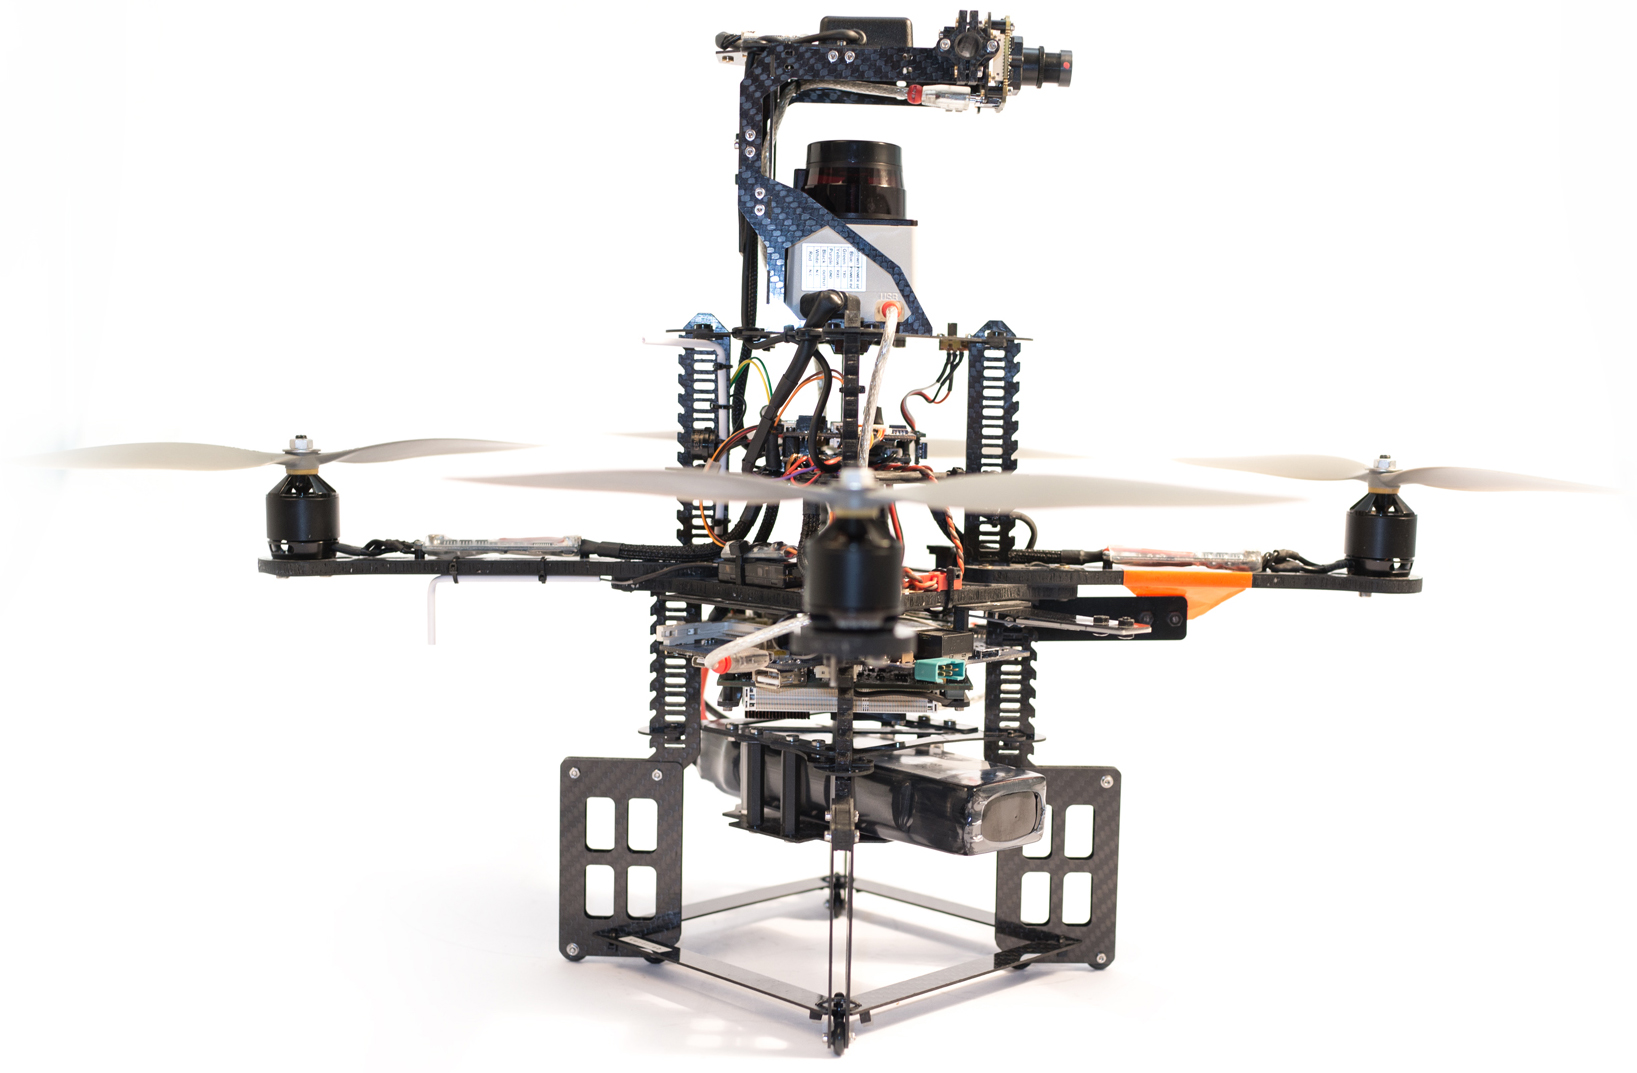
\includegraphics[width=6cm]{img/pelican} &
	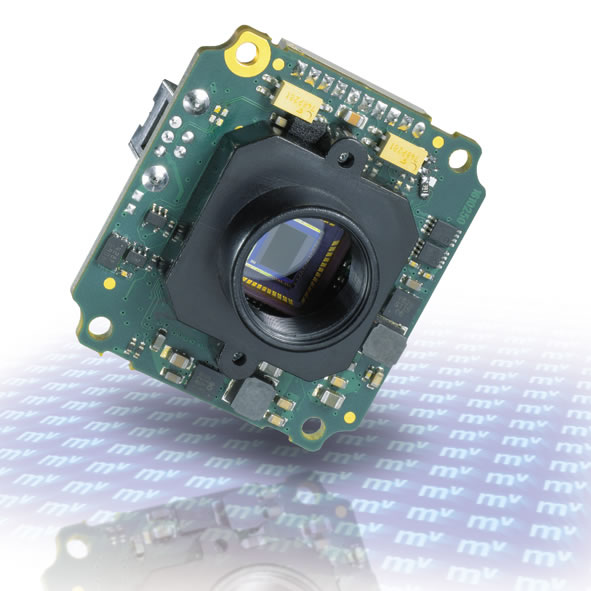
\includegraphics[width=6cm]{img/camera}
	\end{tabular}
	\caption{AscTec Pelikan (links), MatrixVision BlueFOX mv-MLC200wC (rechts)}
	\label{img:pelican}
\end{figure}


\section{Ziel der Arbeit}
\label{sec:ziel_der_arbeit}
Basierend auf photogrammetrischen Konzepten ist es möglich räumliche Tiefe aus zweidimensionalen Bilddaten zu berechnen. Generell werden mindestens zwei Bilder derselben Szene aus unterschiedlichen Standpunkten für die Berechnung dreidimensionaler Informationen benötigt. Bei Verwendung einer einzelnen Kamera muss für ein Bildpaar die relative Orientierung zwischen den Kameras geschätzt werden, wobei keine Information über die Skalierung vorliegt. Bei der Verwendung eines Stereosystems ist die relative Orientierung beider Kameras zueinander bereits bekannt, was eine direkte Berechnung metrischer Koordinaten ermöglicht. Da Zuverlässigkeit sowie Genauigkeit vor allem im Kontext der Navigation in Innenräumen sehr wichtig ist wurde in dieser Arbeit auf ein Stereo-Setup gesetzt.\\

\noindent
Vor diesem Hintergrund werden in Kapitel \ref{chp:concepts} der Arbeit zugrundeliegende Algorithmen und Konzepte erläutert. Weiterhin wird das entwickelte Framework zur Bildaufnahme und Vorprozessierung der Bilder grundlegend beschrieben. Anschliessend werden einige State of the Art Methoden der Hinderniserkennung beschrieben wobei dabei zwischen aktiven und passiven optischen Systemen unterschieden wird. Diese Einteilung dient einerseits dafür einen Überblick über bereits bestehende Techniken sowie implementierte Systeme zu erhalten, andererseits um auch die Vor- und Nachteile der jeweiligen Technik herauszuarbeiten. Im Anschluss daran beschreibt Kapitel \ref{chp:developed_algorithms} die beiden entwickelten Methoden zur bildbasierten Hinderniserkennung und deren Implementierung detailliert. Anschließend erfolgt die Evaluation beider Verfahren wobei die Erkennung verschiedener Hindernisgrößen getestet wird. Weitere Tests hinsichtlich zukünftiger Verbesserungen zeigen auf welches aktuellen Limitierungen durch die verwendeten Konzepte vorliegen. Kapitel \ref{chp:conflicts} erläutert mögliche Ursachen eben dieser Limitierungen und gibt Ansätze zur Lösung aus der Fachliteratur sowie eigene Konzepte zur Bewältigung dieser. Die anschliessende Diskussion wertet die im Rahmen der Evaluation in Kapitel \ref{chp:evaluation} erlangten Ergebnisse weitergehend aus und stellt beide Algorithmen hinsichtlich der Robustheit der Erkennung, sowie der erreichten Performance gegenüber. Kapitel \ref{chp:fazit} zieht ein Ré­su­mé aus den Ergebnissen der Arbeit und gibt einen Ausblick auf mögliche zukünftige Arbeiten in diesem Bereich.